\section{我们的方法}
\label{sec:causalgen-approach}
本节我们首先描述抽取以句子为事件单元因果对的方法。
接着我们阐述因果注意力以及其与软注意力相结合的
融合机制,并将此注意力机制引入到
基于卷积神经网络的序列到序列学习框架中,提高
框架生成质量。
\subsection{因果对的获取}
\label{sec:causalgen-extraction}
基于\secref{sec:causalgen-intro}中的讨论,
本章中我们将句子看作是最基本的描述事件的语义单元,包含\emph{agents}(代理)和\emph{actions}(动作)这两个组成事件的基本要素。
为了学习因果生成任务,我们基于小说文本
\footnote{xxx}构建了
一个新的原因-结果对数据集。
我们从那些包含因果连接词(\emph{because}和\emph{so})抽取主句和从句组成因果对。
\figref{fig:causalgen-parse}中给出了一个具体示例。

\begin{figure}[th]
	\centering
	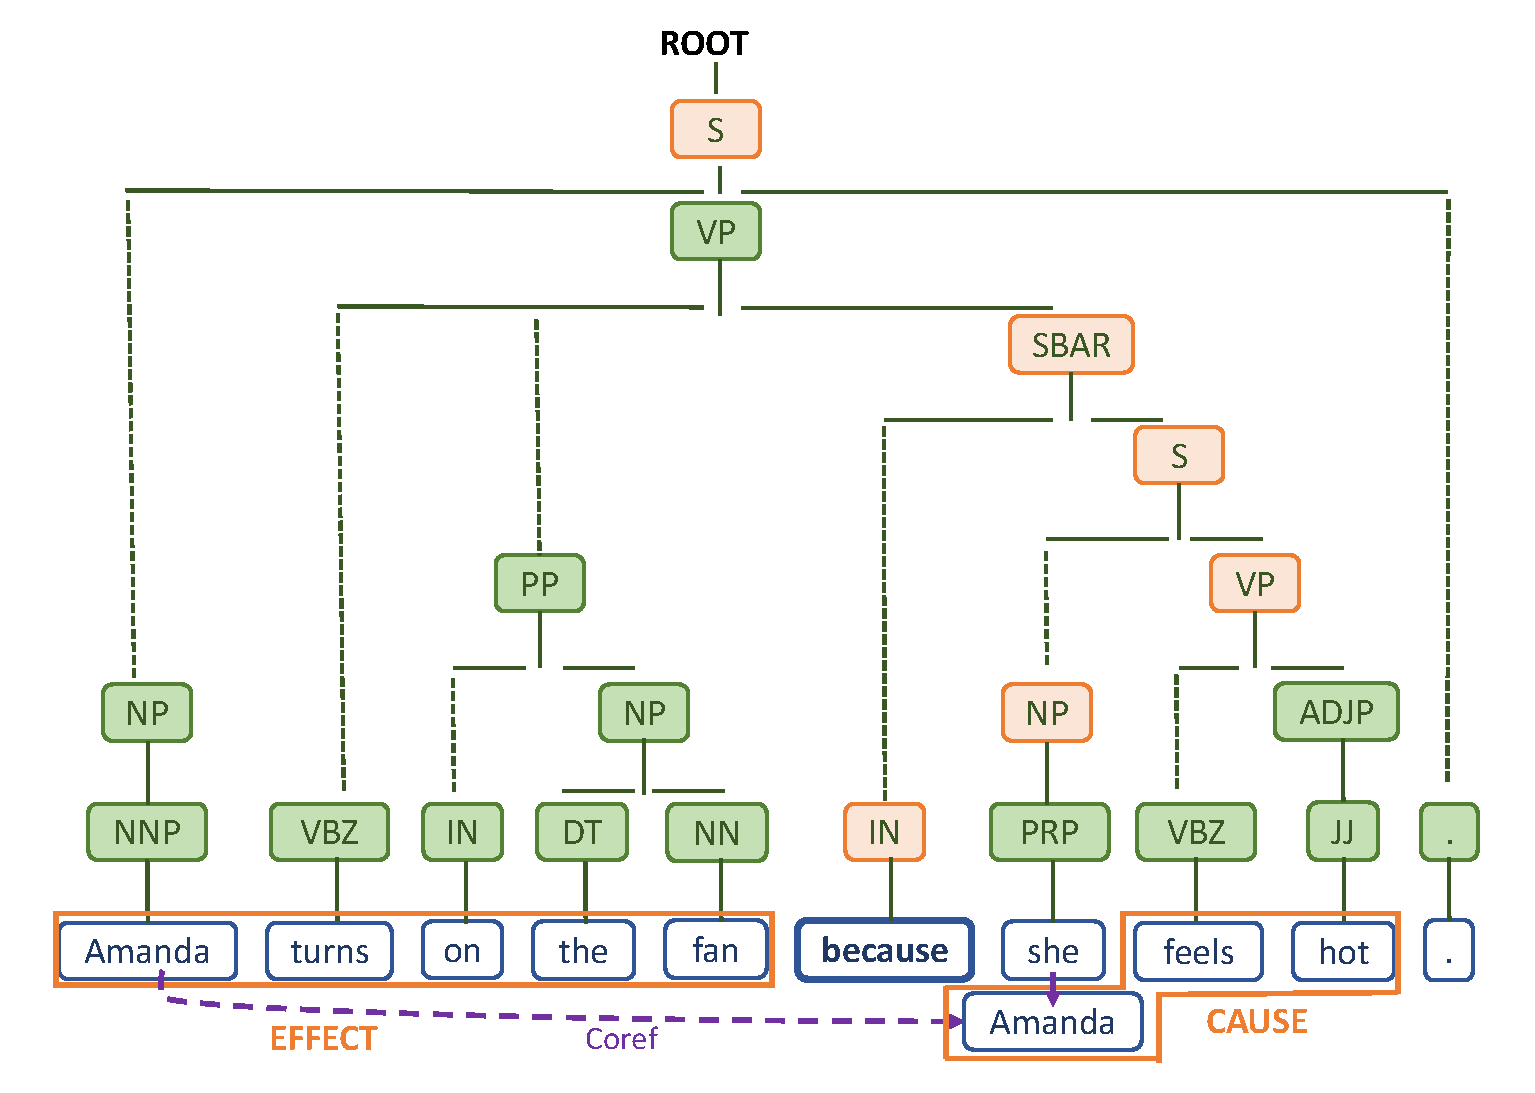
\includegraphics[width=0.8\columnwidth]{figure/causalgen/parse.pdf}
	\bicaption{示例句的句法解析以及抽取因果对的过程展示。树中标记为橙色的结点组成的路径为抽取过程中使用的句法模式。}{Cause and effect sentence extracted from a sample sentence after coreference resolution, along with its constituent parse tree. Nodes coloured in light orange are those critical for syntactical checking in our extraction process.}
	\label{fig:causalgen-parse}
\end{figure}

下面我们详细描述抽取过程涉及的各个步骤:
\begin{itemize}
	\item \emph{句子收集.}~\quad
	我们首先使用正则表达式匹配收集那些含有因果线索连接词\emph{because}或\emph{so}的句子。
	然后,用Stanford CoreNLP~\cite{stanfordcorenlp}工具
	进行分词、标注词性以及句法成分解析和句法依存关系解析。
	\item \emph{否定检测.}~\quad 
	如果因果连接词在依存关系解析树中有否定词\emph{not}或\emph{n't}与其具有\emph{neg}否定依存关系,
	则我们在抽取时不考虑此句子。
	\item \emph{从句检测.}~\quad 
	我们为因果句子对设计句法模式匹配规则。
	我们认为\emph{because}在句中编码因果关系应满足:它在句中引导的从句在成分
	解析树中构成的子树根结点为\emph{SBAR},并包含
	一个陈述子句(以\emph{S}为根且包含主语\emph{NP}
	和谓语\emph{VP})。
	同样地,我们也为\emph{so that}连接词设计了类似的句法规则以便更准确的抽取因果句子对。
	句法规则的使用示例可参见\figref{fig:causalgen-parse}。	
	\item \emph{文本区域抽取.}~\quad
	我们将冗余的标点及不需要的句子成分以删除
	子树的形式从待抽取文本段中去除掉。
	然后,主句子树和从句子树的剩余部分所覆盖的文本区域构成了我们要抽取的因果对。
\end{itemize}

\paragraph*{输入数据格式转换}
我们为每个抽取的因果对构建了两个数据实例,
分别用于正向因果推理和反向因果推理。
在训练阶段,我们在目标文本序列
最前面添加特殊符$\left< f\right>$(或
$\left< b \right>$)表示该数据实例用于
进行正向因果推理(或反向因果推理)。
在测试阶段,我们将生成序列的其实字符
初始化为$\left< f\right>$(或
$\left< b \right>$)以要求模型生成
输入序列的结果(或原因)。
注意,为了给每个因果对创建正向推理和反向推理
的数据实例,我们对包含因果线索连接词的句子做了
指代消解(如\figref{fig:causalgen-parse}所示)。
我们在\figref{fig:causalgen-example}
中展示了\figref{fig:causalgen-parse}中
例句创建的两个数据实例。

\begin{figure*}[th!]
	\centering
	\subfloat[Forward]{
		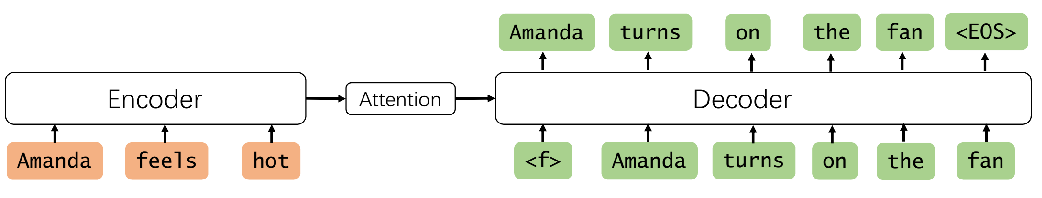
\includegraphics[width=0.8\linewidth]{figure/causalgen/for}
	}
	\quad
	\subfloat[Backward]{
		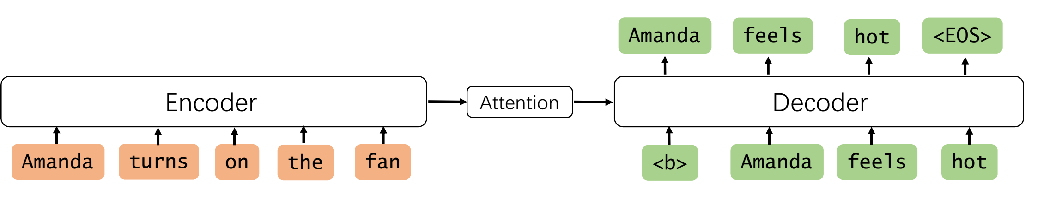
\includegraphics[width=0.8\linewidth]{figure/causalgen/back}
	}
	\bicaption{因果对的正向因果推理和反向因果推理示例。}{The cause-effect pair for forward and backward causal reasoning.}
	\label{fig:causalgen-example}
\end{figure*}

\subsection{基于神经网络的序列到序列模型}
\label{sec:causalgen-cnn}
本节主要介绍基于卷积神经网络的序列到序列
(CNN seq2seq
\footnote{\url{https://github.com/facebookresearch/fairseq-py}})模型框架。
这是我们的一个基线模型,
稍后我们在此基础上实现了本章提出的因果注意力及其融合机制。

在CNN seq2seq模型中,给定输入序列
$\textbf{x} = (x_{1},x_{2},...,x_{m})$ 和输出序列 
$\textbf{y} = (y_{1}, y_{2},..., y_{n})$ ($m>n$),
我们将词嵌入与元素对应的位置嵌入相结合
得到输入状态表示$\mathbf{X} = (X_1,...,X_m)$ 
和输出状态表示 $\mathbf{Y}=(Y_1,...,Y_n)$。
CNN seq2seq框架的编码器和解码器均由
$L$层($L=8$)卷积层层叠而成。
其中,编码器的$l$-th卷积层的输出和解码器的$l$-th卷积层的输出分别记为
$\mathbf { z } ^ { l } = \left( z _ { 1 } ^ { l } , \ldots , z _ { m } ^ { l } \right)$和$\mathbf { h } ^ { l } = \left( h _ { 1 } ^ { l } , \ldots , h _ { n } ^ { l } \right)$。
编码器和解码器中每个卷积层均使用门线性单元~\cite{DauphinFAG17}(GLU)和残差连接~\cite{HeZRS16}等结构,以确保信息在编码器和解码器中进行充分有效的逐层传递,$l$-th层第$i$个位置的输出状态如下:
\begin{equation}
%\small
h _ { i } ^ { l } = ~ GLU \left( W ^ { l } \left[ h _ {i-k/2 } ^ { l - 1 } , \ldots , h _ { i+k/2 } ^ { l - 1 } \right] + b _ { w } ^ { l } \right)  + h _ { i } ^ { l - 1 }
\end{equation} 
,其中\textit{k}为卷积核宽度。

特别地,在解码端
我们对解码器的最后卷积层(即$L$-th解码层)在第$i$个位置的输出状态$h_{i}^{L}$进行线性变换,再利用Softmax函数来计算生成下一个元素$y_{i+1}$的概率分布,计算方法
如\eqnref{eq:causalgen-prob}所示,其中$W _ { o }$和$b_ { o }$是线性变换层的参数。

\begin{equation}
\label{eq:causalgen-prob}
%\small
p \left( y _ { i + 1 } | y _ { 1 } , \ldots , y _ { i } , \mathbf { x } \right) = 
\operatorname { softmax } \left( W _ { o } h _ { i } ^ { L } + b _ { o } \right) \\ 
\in \mathbb { R } ^ { T }
\end{equation}
此外,各解码层还引入了多步注意力机制。
为计算注意力分数,我们先将当前解码状态$h^l_{i}$和之前的生成元素的嵌入表示$Y_i$相结合得到解码状态摘要$d _ { i } ^ { l }$如下:
\begin{equation}
%\small
d _ { i } ^ { l } = W _ { d } ^ { l } h _ { i } ^ { l } + b _ { d } ^ { l } + Y _ { i }
\end{equation}
其中$W _ { d }$和$b_ { d }$是线性变换层的参数。
对于$l$解码层,我们计算$d _ { i } ^ { l }$与最后编码层(即$L$编码层)的第$j$个输入元素的编码输出状态$z^L_j$的点积,得到解码状态第$i$输出和第$j$输入元素之间的注意力分数$a^l_{ij}$,如\eqnref{eq:causalgen-attn-a}所示,其中$\sum_{ t = 1 }^{m}a_{it} = 1$,$a _ { i j }$在0-1之间取值。
\begin{equation}
\label{eq:causalgen-attn-a}
%\small
a _ { i j } ^ { l } = \frac { \exp \left( d _ { i } ^ { l } \cdot z _ { j } ^ { L } \right) } { \sum _ { t = 1 } ^ { m } \exp \left( d _ { i } ^ { l } \cdot z _ { t } ^ { L } \right) }
\end{equation}

我们将编码状态$z_j^L$与输入表示$X_j$相结合,
并利用\eqnref{eq:causalgen-attn-a}中得到的注意力分数对其进行加权求和得到对输入上下文的摘要表示向量$c _ { i } ^ { l }$。
$c _ { i } ^ { l }$计算如下:
\begin{equation}
\label{eq:causalgen-attn-c}
c _ { i } ^ { l } = \sum _ { j = 1 } ^ { m } a _ { i j } ^ { l } \left( z _ { j } ^ { L } + X_j \right)
\end{equation}
,再将 $c _ { i } ^ { l }$与当前解码层输出状态$h_{i}^{l}$相加做为下一解码层的输入。

\subsection{因果注意力模型}
\label{sec:causalgen-causal-attention}
我们在\secref{sec:causalgen-extraction}中
获取的因果对组成的数据集上训练序列到序列模型,
用于因果生成。虽然我们
使用\emph{because}和\emph{so}等置信度较高
的因果线索连接词、设计句法模式等一系列措施
来提高因果对的精度,
但由于因果关系的复杂性和歧义性等特点,
高精度的训练资源仍然十分匮乏。
我们设计因果注意力机制,为模型引入外部因果知识,以提高模型因果生成的效力,弥补训练数据在数量和精度上的劣势。
我们使用我们在\chapref{chap:causalnet-main}中
提出的因果关系网络CausalNet~\cite{luo2016commonsense}作为
外部因果知识库,在因果生成时为模型提供
全局的因果依存关系信息。

由\chapref{chap:causalnet-main}的工作描述可知,
CausalNet是一个网络规模( web-scale)的
因果关系网络,蕴含大量因果关系。
而\secref{sec:causalnet-strength}中提出的因果强度度量$CS$方法具有推理常识因果依存关系的能力。
在Seq2Seq框架中,我们将
因果依存关系建模成一种因果语义上的对齐
机制。具体地,我们利用对数空间下的
词级别(word-level)
间因果关系强度(即$CS$度量)
作为因果注意力分数,
这是由于$CS$指权相乘的定义方式。

我们不妨以正向推理为例讨论模型设计,
即输入为原因,生成目标为结果。
那么,输出序列的$y_i$作为结果中的词
(记为${y_i}_e$)
与输入序列的$x_i$作为原因中的词(
记为${x_j}_c$),
它们之间的因果关系强度的对数形式计算如下:
\begin{equation}
\label{eq:causalgen-acs}
CS({x_j}_c, {y_i}_e) = \log\left(cs({x_j}_c, {y_i}_e)\right) - \log\left(min\{cs({\cdot}_c, {\cdot}_e)\}\right)
\end{equation}
类似地,反向推理时,只需将输入序列作为结果,生成输出序列作为原因即可。
我们在\secref{sec:causalgen-extraction}中介绍了输入数据格式的转换方式以便模型能够区分出当前需要进行正向推理还是反向推理。

对于朴素因果注意力机制,我们尝试
用$Softmax\left( CS({x_j}_c, {y_i}_e)\right)$
替换原模型中\eqnref{eq:causalgen-attn-a}所示
的软注意力分数$a^l_{ij}$。
但这样做存在一个问题,
我们可以看到,
传统的软注意力分数$a^l_{ij}$
是根据当前解码状态摘要$d^l_i$
与编码器状态$z^l_j$计算得到的,
但因果注意力分数$CS({x_j}_c, {y_i}_e)$
并不是基于隐含状态得到的。
在$i$-th时间步解码时,
为计算$CS({x_j}_c, {y_i}_e)$,
我们需要从因果知识库中检索
$({x_j}_c, {y_i}_e)$的因果共现次数等信息,
这要求我们要预先知道源词$x_j$与目标词$y_i$
是什么。这在训练阶段并不困难,
因为我们预先知道标准生成答案(golden targets),
然而在测试阶段我们并不能预先知道真正的
目标词是什么。
我们训练一个加权向量$\mathbf{w_p}$,
对所有目标候选词$y_{\cdot} \in V^t$
($V^t$为目标词汇集)
与源词$x_j$形成的因果强度
$CS({x_j}_c, {y_{\cdot}}_e)$
进行加权平均以得到模型的因果注意力分数
$ca^{l} _ { i j }$:
\begin{equation}
\label{eq:causalgen-ca} 
ca^{l} _ { i j }= \mathbf{w_p} \cdot
\mathbf{cs}(x_j) ,
\end{equation}
其中$\mathbf{cs}(x_j)$是因果强度向量,
它的$i$-th元素的值是$CS({x_j}_c, {V^t_i}_e)$。
我们用\eqnref{eq:causalgen-ca}中的$ca^{l} _ { i j }$
代替\eqnref{eq:causalgen-attn-a}中的$a^l_{ij}$,
将因果注意力机制融入序列到序列学习框架中,
这就是我们的因果注意力基线模型,
在后面实验中记为CAttn。


\subsection{注意力融合机制}
\label{sec:causalgen-fusion}
在\secref{sec:causalgen-causal-attention}中我们
利用CausalNet设计了因果注意力机制,
在因果生成中引入了全局因果知识。
然而,但这种全局性的因果关系映射
只与词项有关,
不论何时对于相同词项,第一解码层和编码层的注意力
都会被赋为基于全局因果强度的因果注意力分数,
这会在一定程度上破坏之前学习到的分布,
也使得模型失去了层次化的语义注意力信息。
而软注意力机制可以学习到局部的语义依存关系,
并在网络层之间逐层传递。
因此,我们提出了一种注意力融合机制
将因果注意力与层叠的软注意力相结合进行因果生成。
该因果注意力融合机制的具体结构如\figref{fig:causalgen-fusedatt}所示。
下面我们具体描述这一注意力融合机制。

\begin{figure*}[th]
	\centering
	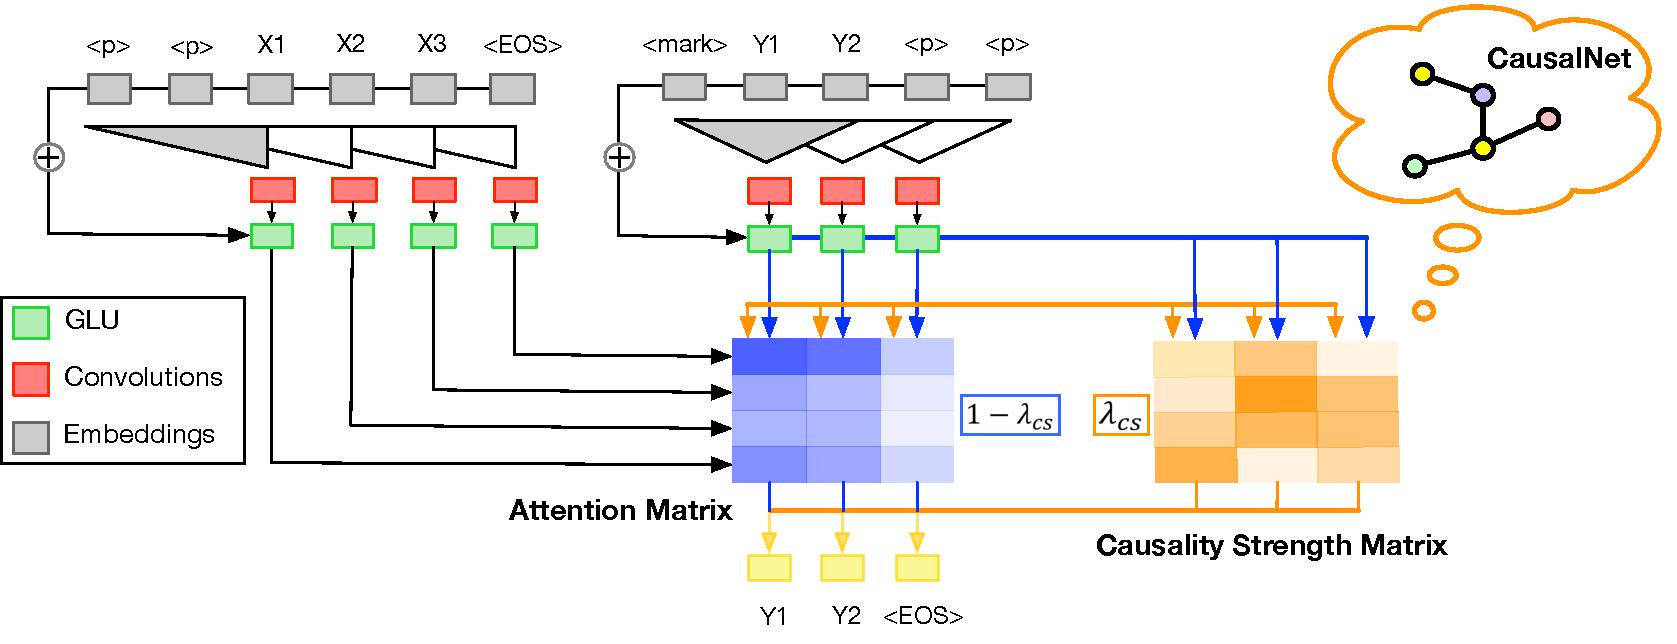
\includegraphics[width=0.95\columnwidth]{figure/causalgen/fusedatt2}
	\bicaption{因果注意力融合机制}{Causal attention fusion mechanism. }
	\label{fig:causalgen-fusedatt}
\end{figure*}

软注意力和\secref{sec:causalgen-causal-attention}中
提出的因果注意力分别从局部和全局的角度编码了
输入源文本与目标文本之间蕴含的因果依存关系。
为了增强模型的表达能力,
我们使用加权方法将全局因果依存信息与局部因果依存信息
相融合。
我们通过因果融合权重(causal fusion weight)
$\lambda_{cs}$对因果注意力分数$ca^l_{ij}$和软注意力
分数$sa^l_{ij}$进行加权得到融合之后的注意力分数
$fa^l_{ij}$如下:
\begin{equation}
\label{eq:causalgen-fusion}
fa^l_{ij} = \lambda^{l}_{cs} \cdot ca^l_{ij} + (1-\lambda^{l}_{cs}) \cdot sa^l_{ij},
\end{equation}
其中$\lambda^{l}_{cs}$表示因果注意力的权重,
用于调节全局因果依存信息对模型的影响力。
\eqnref{eq:causalgen-attn-a}和\eqnref{eq:causalgen-ca}
分别展示了$sa^l_{ij}$和$ca^l_{ij}$的计算方法。
我们计算$\lambda^l_{cs}$的方法如下:
\begin{equation}
\label{eq:causalgen-weight}
\lambda^l_{cs} = \sigma(w^l),
\end{equation}
其中,$\sigma$表示sigmoid函数,
将$\lambda^l_{cs}$映射到0-1之间,
$w^l$是模型中可学习参数。
我们将$l$-th层的因果融合权重
$\lambda^l_{cs}$
作为可训练参数使得融合机制更灵活。

%\subsection{模型精化过程}
%\label{sec:causalgen-finetune}












	